% !TEX root = ../main.tex

\section{Pair Measurement}
\label{sec:pair-measurement}

\scaffold{
  \textbf{Paragraph 1, the drive states.} The star point is not accessible, so the arms have to be inferred from the contacts. Every contact can be connected to a pull-up resistor to the high rail, to a pull-down resistor to the low rail, or left floating, and every contact is read by the ADC (\cref{fig:pull-matrix}). Define the term \emph{reading}: one settled ADC result of one contact; its cost in time follows in \cref{sec:conversion}. Define the term \emph{drive} (high, low, floating) and the term \emph{pull resistance} $R_\mathrm{p}$; on this board $R_\mathrm{p} = \qty{1}{\kilo\ohm}$ for both rails. Define \emph{rail voltages} $V_{\mathrm{H},i}$ and $V_{\mathrm{L},i}$: what contact $i$ reads when it is driven high or low while no current flows. They are measured, not assumed, by driving all three arms to the same rail and averaging eight readings per arm; this cancels the offset of the ADC and the voltage drops of the switches.
}

\begin{figure}[htbp]
  \centering
  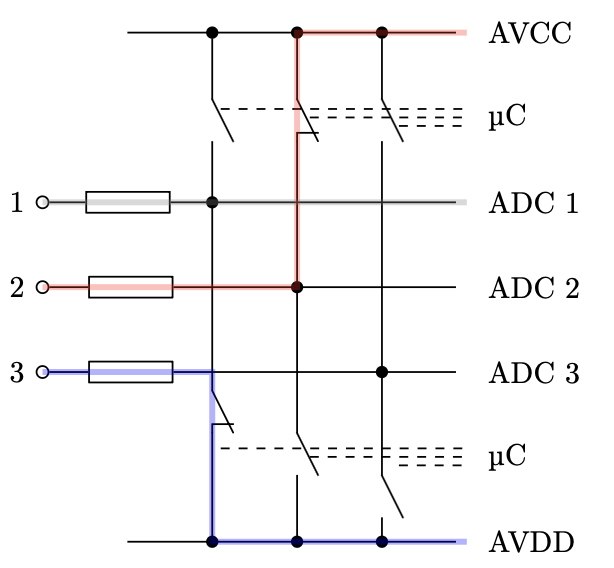
\includegraphics[width=0.45\linewidth]{03-measurement-principle/figures/pull-matrix}
  \titledcaption{Pull Matrix}{\scaffoldinline{Explain the three switch columns per contact (to the high rail, to the low rail, each controlled by the microcontroller), the series resistor at each contact and the ADC channel per contact. The highlighted example drives contact 2 high and contact 3 low while contact 1 floats. Note that the figure labels the rails AVCC and AVDD; in the text they are the high and low rail.}}
  \label{fig:pull-matrix}
\end{figure}

\scaffold{
  \textbf{Paragraph 2, one pair.} A \emph{pair measurement} drives one arm $h$ high and one arm $l$ low and leaves the third arm $f$ floating, then reads all three contacts. The floating contact carries no current, so it reads the star point voltage. Present \cref{eq:currents,eq:pair-resistance,eq:low-fraction} in this order and explain each in one sentence: the loop current seen on the high and on the low side, the resistance of the pair, and the share of the pair held by the low arm. Point out that \cref{eq:low-fraction} uses voltages only, which span most of the rail, while \cref{eq:currents} relies on the small drops across the pull resistors; this is why ratios are precise and the total is not.
}

\begin{align}
  I_\mathrm{H} &= \frac{V_{\mathrm{H},h} - V_h}{R_\mathrm{p}},
  \qquad
  I_\mathrm{L} = \frac{V_l - V_{\mathrm{L},l}}{R_\mathrm{p}},
  \qquad
  I = \frac{I_\mathrm{H} + I_\mathrm{L}}{2}
  \label{eq:currents} \\
  R_{hl} &= r_h + r_l = \frac{V_h - V_l}{I}
  \label{eq:pair-resistance} \\
  \rho_{hl} &= \frac{V_f - V_l}{V_h - V_l} = \frac{r_l}{r_h + r_l}
  \label{eq:low-fraction}
\end{align}

\scaffold{
  \textbf{Paragraph 3, consistency and conduction.} $I_\mathrm{H}$ and $I_\mathrm{L}$ are two readings of the same loop current, so their difference is a free consistency check: a pedal moved during the measurement, or an unsettled contact, shows up as disagreement. A pair conducts only if both driven arms are finite; an isolated arm leaves $I$ at zero within the noise. Refer forward to \cref{sec:tolerances} for the thresholds of both checks.
}

\scaffold{
  \textbf{Paragraph 4, worked example.} Walk through \cref{fig:topology-sim-pairs}: the simulator of milestone~2 \cite{benson2026topologysim} with arms of 100, 200 and \qty{300}{\kilo\ohm} and \qty{1}{\kilo\ohm} pulls. In (a), the first pair puts the floating contact at \qty{1.66}{\volt}, i.e. 67\,\% of the span; in (b) the second pair puts it at \qty{1.87}{\volt}, 75\,\%. Compute both ratios with \cref{eq:low-fraction} to show the reader the arithmetic once. Mention that the simulator assumes a \qty{2.5}{\volt} rail.
}

\begin{figure}[htbp]
  \centering
  \begin{subfigure}[t]{0.49\linewidth}
    \centering
    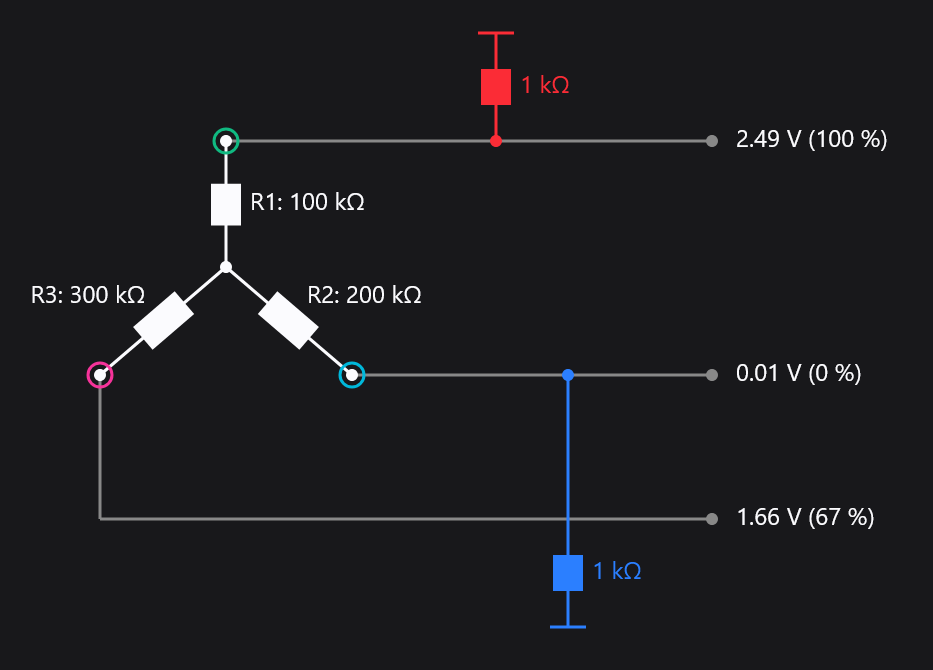
\includegraphics[width=\linewidth]{03-measurement-principle/figures/topology-sim-first-pair}
    \caption{First Pair}
    \label{fig:topology-sim-first-pair}
  \end{subfigure}%
  \hfill%
  \begin{subfigure}[t]{0.49\linewidth}
    \centering
    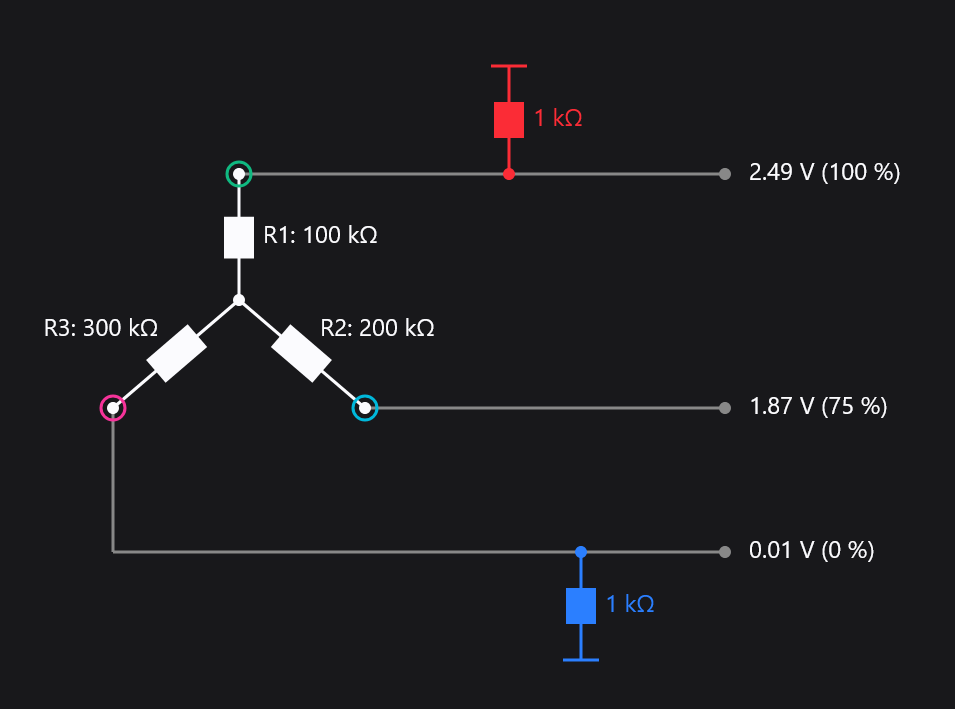
\includegraphics[width=\linewidth]{03-measurement-principle/figures/topology-sim-second-pair}
    \caption{Second Pair}
    \label{fig:topology-sim-second-pair}
  \end{subfigure}
  \titledcaption{Pair Measurements in the Simulator}{\scaffoldinline{State the network (R1 \qty{100}{\kilo\ohm}, R2 \qty{200}{\kilo\ohm}, R3 \qty{300}{\kilo\ohm}), mark which contact is pulled up (red) and down (blue) in (a) and (b), and read off the floating contact voltage in each. Screenshots of \cite{benson2026topologysim}; verify that the arm labels match the text before use.}}
  \label{fig:topology-sim-pairs}
\end{figure}
